\section{Mega Examples}

in some cases, one needs combined knowledge from several sections to solve a problem

in this section, we walk through a few long questions to consolidate thinking

\example{A particle $P$ of mass $m$ rests on a smooth horizontal table, and is connected to a fixed point $A$ by an elastic string of natural length $2a$ and modulus of elasticity $mg$. When the particle is at its rest position $O$, it is given an impulse of magnitude $m\sqrt{\frac{ga}{2}}$ and $P$ starts to move away from $A$ towards a barrier $B$. The barrier is at a distance of $\frac{1}{2}a$ from $O$. The coefficient of restitution between the particle and the barrier is $\frac{1}{\sqrt{3}}$. Find the time when $P$ first returns to $O$.}

\begin{figure}[htp]
	\begin{center}
		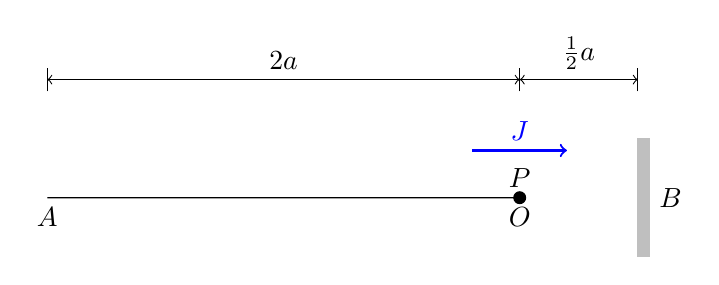
\begin{tikzpicture}[scale=1.5]
		\draw[fill] (0,0)node[below]{$A$} -- (4,0) circle(0.05) node[above]{$P$} node[below]{$O$};
		\draw[gray!50,fill] (5,-0.5) rectangle (5.1,0.5);
		\node[right] at (5.1,0) {$B$};
		\draw[<->] (0,1) -- (4,1) node[midway, above]{$2a$};
		\draw[<->] (4,1) -- (5,1) node[midway, above]{$\frac{1}{2}a$};
		\draw (0,0.9) --++ (0,0.2);
		\draw (4,0.9) --++ (0,0.2);
		\draw (5,0.9) --++ (0,0.2);
		\draw[blue,thick,->] (3.6,0.4) --++ (0.8,0) node[midway, above]{$J$};
		\end{tikzpicture}
	\end{center}
\end{figure}

motion of $P$ consists of three stages: motion from $O$ to $B$ (part of simple harmonics), impact with barrier, and motion from $B$ to $O$ (also simple harmonic, but with a different amplitude)

we first write down the equation of motion when $OP = x$, :

{

\centering

$m\ddot{x} = -\frac{\lambda}{l_0}x \RA m\ddot{x} = -\frac{mg}{2a}x \RA \ddot{x} = -\frac{g}{2a}x$

}

so $P$ describes simple harmonic motion along $OB$ with angular frequency $\omega = \sqrt{\frac{g}{2a}}$

at $t=0$, impulse-momentum relation reads: $J=m\sqrt{\frac{ga}{2}}=mu_0 \RA u_0 = \sqrt{\frac{ga}{2}}$

from $O$ to $B$, amplitude of motion is: $x_0 = \frac{u_0}{\omega} = \sqrt{\frac{ga}{2}} \cdot \sqrt{\frac{2a}{g}} \RA x_0 = a$

displacement-time relation is: $x(t)=x_0\sin\omega t \RA x(t)=a\sin\omega t $

just before hitting barrier, $x=\frac{1}{2}a$, so

{

\centering

$a\sin\omega t_1 = \frac{1}{2}a \RA \omega t_1 = \sin^{-1}\tfrac{1}{2} \RA t_1 = \frac{\pi}{6\omega}$

$u = \omega\sqrt{x_0^2-x^2} = \sqrt{\frac{g}{2a}} \cdot \sqrt{a^2-\frac{1}{4}a^2} \RA u=\sqrt{\frac{3ga}{8}}$

}

after hitting barrier: $v = -eu = -\frac{1}{\sqrt{3}}\cdot \sqrt{\frac{3ga}{8}} \RA v = -\sqrt{\frac{ga}{8}}$

{
	
\centering
	
$v^2 = \omega\sqrt{x_0^2-x^2} \RA x'_0 = \sqrt{\frac{v^2}{\omega^2} + x^2} = \sqrt{\frac{ga}{8} \cdot\ \frac{2a}{g} + \frac{1}{4}a^2} \RA x'_0 = \frac{1}{\sqrt{2}}a$

}

so as $P$ travels from $B$ back to $O$, amplitude becomes smaller

note that it takes the same time for $P$ to move from $O$ to $B$ as long as amplitude is fixed

we can use displacement-time relation $x'(t)=x'_0\sin\omega t$, or  $x'(t)=\frac{1}{\sqrt{2}}a\sin\omega t$, to find:

{
	
\centering
	
$ \frac{1}{\sqrt{2}}a\sin\omega t_2 = \frac{1}{2}a \RA \omega t_2 = \sin^{-1}\tfrac{1}{\sqrt{2}} \RA t_2 = \frac{\pi}{4\omega}$
	
}

total time taken: $t=t_1+t_2 = \frac{\pi}{6\omega}+\frac{\pi}{4\omega} = \frac{5\pi}{12\omega} \RA t=\frac{5\pi}{12} \sqrt{\frac{2a}{g}}$ \eoe
	
\example{A uniform disc of radius $a$ and mass $2m$ is free to rotate in a vertical plane about a horizontal axis through its centre $O$. A particle $P$ of mass $m$ is placed on the highest point of the rough edge of the disc. The system is slightly disturbed so that $OP$ begins to rotate. For the subsequent motion, the particle remains in contact with the disc without slipping. (a) When OP makes an angle $\theta$ with the upward vertical, find $\dot{\theta}$ and $\ddot{\theta}$ in terms of $g$ and $\theta$. (b) Given that the coefficient of friction between the particle and the disc is $\mu=\frac{1}{4}$, find the angle $\theta$ when $P$ just begins to slip. (c) Show that, however large the value of $\mu$, the particle cannot lose contact with the disc before it starts to slip.}

\begin{figure}[htp]
	\begin{center}
		\begin{tikzpicture}[scale=0.8]
		\draw (0,0) node[below]{$O$} circle(4);
		\draw[dashed] (0,4) -- (0,0) node[midway,left]{$a$} -- (60:4) node[midway,right]{$a$};
		\draw[fill] (60:4.1) circle(0.1) node[right]{$P$};
		\node at (75:1.1) {$\theta$};
		\draw (0,0.8) arc(90:60:0.8);
		\draw[blue,thick,->] (60:4.1) --++ (0,-2.5) node[right]{$mg$};
		\draw[blue,thick,->] (60:4.1) --++ (60:1.5) node[right]{$N$};
		\draw[blue,thick,->] (60:4.1) --++ (150:1) node[above]{$f$};
		\end{tikzpicture}
	\end{center}
\end{figure}

\vspace*{-0.5\baselineskip}

moment of inertia of system is:

{
	
	\centering
	
	$I = I_\text{disc} + I_P = \frac{1}{2}\cdot2ma^2 + ma^2 \RA I = 2ma^2$
	
	
}

to find $\dot{\theta}$, consider energy changes, loss in G.P.E. for particle becomes rotational K.E. of system:

{

\centering

$mga(1-\cos\theta) = \frac{1}{2}I\dot{\theta}^2 \RA mga(1-\cos\theta) = \frac{1}{2} \cdot 2ma^2 \cdot \dot{\theta}^2 \RA \dot{\theta}^2 = \frac{g(1-\cos\theta)}{a} $

}

to find $\ddot{\theta}$, consider torque acting on system:

{

\centering

$\tau = I\ddot{\theta} \RA mga\sin\theta = 2ma^2\cdot\ddot{\theta} \RA \ddot{\theta} = \frac{g\sin\theta}{2a}$

}

or one can take time derivative for $\dot{\theta}^2$ to find:

{

\centering

$\ddt{\dot{\theta}^2} = \opdt\left(\frac{g(1-\cos\theta)}{a}\right)  \RA 2\dot{\theta}\cdot\ddot{\theta} = \frac{g\sin\theta\cdot\dot{\theta}}{a} \RA \ddot{\theta} = \frac{g\sin\theta}{2a}$

}

to find friction and contact force on $P$, consider tangential and centripetal forces on $P$:

{

\centering

$mg\sin\theta - f = m\cdot a\ddot{\theta} \RA f = mg\sin\theta - m\cdot \frac{1}{2}g\sin\theta \RA f= \frac{1}{2}mg\sin\theta$

$mg\cos\theta - N = m\dot{\theta}^2 a \RA N = mg\cos\theta - mg(1-\cos\theta) \RA N = mg(2\cos\theta -1) $ ($\Delta$)

}

when $P$ is about to slip, frictional force is at limiting value $f=\mu N$

{

\centering

$\frac{1}{2}mg\sin\theta = \mu mg(2\cos\theta -1) \RA \sin\theta = 4\mu\cos\theta -2\mu \RA 4\mu\cos\theta -\sin\theta = 2\mu$ (\#)

}

to find limiting $\theta$, substitute $\mu=\frac{1}{4}$, we find

{

\centering

$\cos\theta - \sin\theta = \frac{1}{2} \RA \sqrt{2}\cos(\theta+45^\circ)=\frac{1}{2} \RA \theta = \cos^{-1}\tfrac{1}{2\sqrt{2}} - 45^\circ \RA \theta \approx 24.3^\circ$

}

rewrite (\#) as $\cos\theta = \frac{2\mu+\sin\theta}{4\mu}$, and plug this into ($\Delta$):

{

\centering

$N = mg\left(2\cdot \frac{2\mu+\sin\theta}{4\mu} - 1\right) = mg\left(1 + \frac{\sin\theta}{2\mu} -1 \right) \RA N = \frac{mg\sin\theta}{2\mu}$

}

obviously $N>0$, so $P$ will not lose contact before slipping occurs \eoe